%% The first command in your LaTeX source must be the \documentclass command.
\documentclass[sigconf,authorversion]{acmart}
%% NOTE that a single column version may be required for
%% submission and peer review. This can be done by changing
%% the \doucmentclass[...]{acmart} in this template to
%% \documentclass[manuscript,screen,review]{acmart}

\begin{document}
\settopmatter{printacmref=false}
\setcopyright{none}
\renewcommand\footnotetextcopyrightpermission[1]{}
\pagestyle{plain}
\title{Modeling the Latent Space of Symbolic String Quartet Music}

%%
%% The "author" command and its associated commands are used to define
%% the authors and their affiliations.
%% Of note is the shared affiliation of the first two authors, and the
%% "authornote" and "authornotemark" commands
%% used to denote shared contribution to the research.

\author{Alex Kyllo}
\email{akyllo@uw.edu}
\affiliation{%
  \institution{University of Washington}
  \city{Bothell}
  \state{WA}
  \country{USA}
}

\begin{abstract}
  This paper presents the results of a project to apply a recurrent
  variational autoencoder to the task of modeling a latent space for
  generating pieces of multi-instrument symbolic classical music
  through interpolation.
\end{abstract}

\keywords{deep learning, recurrent neural networks, sequential models,
  music modeling, latent space modeling, generative modeling}

\maketitle

\section{Introduction}

Machine learning models of music have interesting applications in
music information retrieval and creative tools for musical artists and
educators. Generative models can create accompaniments for music,
blend and transfer styles between clips of music, and even generate
entirely new music. Music is challenging to model because it is
inherently high-dimensional, exhibiting a complex hierarchy of
recurring patterns and long-range temporal dependencies, and because
musical scores have multiple possible digital representations with
distinct advantages and disadvantages.

Depending on the task, machine learning models of music may be trained
on the audio signal of a musical performance, either in a time domain
or a frequency domain representation, or they may be trained on a
digital symbolic representation of music, the most common of which is
MIDI (Musical Instrument Digital Interface) notation. MIDI is an
encoding of music as streams of bytes in one or more tracks or
channels, each representing a sequence of 128 possible pitch values
(where 0 is the lowest pitch and 127 is the highest), along with
timing, pressure and instrument identifier values. A generative
symbolic music model can produce a symbolic score in MIDI format,
which must be played by synthesizer software or by humans to produce
an audio music performance. This project focuses on generative
modeling of symbolic (MIDI) music to compose original musical scores
by blending input scores through continuous latent space interpolation.

\section{Related Work}

The state of the art in music generation still has a long way to go
before it can consistently generate music scores or performances that
would be enjoyable and popular for humans to listen to, but for this
reason it is an area of significant opportunity, where a number of
recent research projects have shown promising progress.

Google's \href{https://magenta.tensorflow.org/}{Magenta} is an
umbrella project for music deep learning research and development of
software tools to expose these models for use by creative artists and
students.

MusicVAE, part of the Magenta project, is a variational Long
Short-Term Memory (LSTM) autoencoder for MIDI that incorporates a
novel hierarchical structure using a ``conductor'' recurrent layer in
its decoder model to better capture structure at multiple levels and
avoid the problem of ``posterior/mode collapse'' whereby a generative
model learns to ignore its latent code and rely on autoregression
\cite{roberts_hierarchical_2018}. This model is trained on 16-bar
paragraphs of music and is capable of generating new melodies that
blend two given melodies via latent space interpolation.

Another Magenta model called Music Transformer is a generative model
that borrows its approach from the Natural Language Processing (NLP)
domain, using a self-attention network to model MIDI music as a
sequence of discrete tokens with relative positional dependencies
\cite{huang_music_2018}. The focus of this model is on learning
long-term dependencies in music to produce longer clips of music with
coherent structure. Music Transformer was trained on a dataset of
Piano-e-competition performances \cite{hawthorne2019enabling} and its
generated piano music received favorable qualitative (Likert scale)
ratings from human listeners for its resemblance to human-composed
music \cite{huang_music_2018}.

MuseGAN \cite{dong2017musegan} is an application of Generative
Adversarial Networks (GAN) to polyphonic MIDI music generation,
trained on four-bar phrases of a multi-track pianoroll representation
of rock songs from the Lakh Midi Dataset
\cite{raffel_learning-based_2016}. Like MusicVAE, MuseGAN includes a
two-level generator that first samples latent codes at the phrase or
bar level, then generates notes within the bars, to produce
longer-term structural patterns.

\begin{figure}[h]
  \centering
  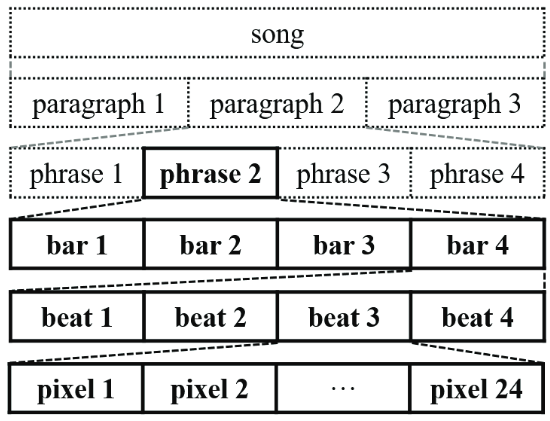
\includegraphics[width=\linewidth]{song_structure.png}
  \caption{Diagram of the hierarchical structure of a musical
    composition, from the MuseGAN paper \cite{dong2017musegan}.}
  \label{song_structure}
  \Description{A diagram showing the hierarchical structure of songs,
    to paragraphs, to phrases, to bars, to, beats, to pixels.}
\end{figure}

A major advantage of working with the symbolic representation of music
is that it is of far lower dimensionality than the raw audio waveforms
of a recorded performance, which makes it less computationally
expensive. However, there are many stylistic aspects of musical
performance that are not captured by a symbolic representation, and
may be specific to a particular performer, so the expressiveness of
symbolic generative models is limited in comparison
\cite{manzelli_conditioning_2018}.

Other research has focused on modeling raw audio waveforms directly. WaveNet is
a causal convolutional neural network for generating raw audio waveforms,
developed by Google DeepMind, which achieves state of the art performance in
generating natural sounding speech from text, but is also capable of generating
short, realistic snippets of audio music \cite{oord_wavenet_2016}.
Another model named SampleRNN generates raw audio waveforms using a three-tier
hierarchy of gated recurrent units (GRU) to model recurrent structure at
multiple temporal resolutions \cite{mehri_samplernn_2017}.

Prior work points out that the division between symbolic music notes
and music performances, is analogous to the division between symbolic
language and utterances in speech, which may inspire ideas for
combining the two approaches \cite{hawthorne2019enabling}. A paper
from Boston University describes an effort to combine the symbolic and
waveform approaches to music modeling, by training an LSTM to learn
melodic structure of different styles of music, then providing
generations from this model as conditioning inputs to a WaveNet-based
raw audio generator \cite{manzelli_conditioning_2018}.

\section{Methods}

\subsection{Datasets}

The dataset used for this research project is MusicNet, which is a
collection of 330 freely licensed European classical music recordings
with aligned MIDI scores \cite{thickstun2017learning}.  The model is
trained on 36 string quartets (four-part arrangements with two
violins, one viola and one cello) by composers Bach, Beethoven,
Dvorak, Haydn, Mozart, and Ravel.

\subsection{Data Preprocessing}

Several choices must be made in how to preprocess binary MIDI files
into training examples for a neural network. There are multiple
open-source Python packages that assist with the process of reading
MIDI files from their binary on-disk representations into Python
objects, such as pretty\_midi \cite{raffel_pretty_midi_2014},
Pypianoroll \cite{dong_pypianoroll_2018} and music21
\cite{cuthbert_music21_2010}.

In order to accommodate polyphonic music, we each MIDI file is
converted into a modified pianoroll representation, an example of
which is visualized in Figure \ref{pianoroll}. In this modified
representation, each instrument track is a sequence of integers from
0-129 representing the MIDI note pitch value being played at the given
time step, where values 0-127 are pitches, 128 is a rest (silence) and
129 is sustain, indicating that the previously played pitch is held
continuously. Because chords (multiple notes being played
simultaneously by the same instrument) are relatively rare in string
quartets, the lowest note of each chord is taken and the rest
discarded, to reduce dimensionality. Because notes at the extreme low
and high end are rare and are out of range of common instruments, the
note pitch values are clipped to a narrower range and ordinal
encoded. For the 36 string quartets found in the MusicNet database,
this results in 66 distinct values, where 0-63 represent notes played
by the violins, viola and cello, 64 is rest and 65 is sustain. Our
software package also includes functions to convert this
representation back into a Music21 Score object, which can then be
written to a MIDI file.

Because songs are typically at least a few minutes long and of varying
length, it will not be feasible to train with entire songs as
examples, so we will crop songs into phrases of equal numbers of
measures to use as training data.

The result of this preprocessing is that each training example isbe a
2D matrix of shape (time steps x instrument tracks) and stacking the
training examples produces a 3D tensor. Information regarding which
track corresponds to which musical instrument is lost and therefore
must be maintained separately to reconstruct the MIDI
representation. For string quartets this instrument ensemble is always
\texttt{[40, 40, 41, 42]}, which is an array of MIDI instrument codes
representing two violins, one viola and one cello. Tempo information
is also lost from this representation, so the outputs are normalized
to the default tempo of 120 beats per minute.

As the model will produce one output per instrument track, it can
incorporate only a fixed selection of instrument parts, similar to how
MusicVAE models three-part (drum, bass and melody)
\cite{roberts_hierarchical_2018} and MuseGAN models five-part (drum,
bass, guitar, string, piano) arrangements. Therefore this model is
purpose-built for string quartets, which are the most common type of
arrangement found in the MusicNet dataset.

\begin{figure}[h]
  \centering
  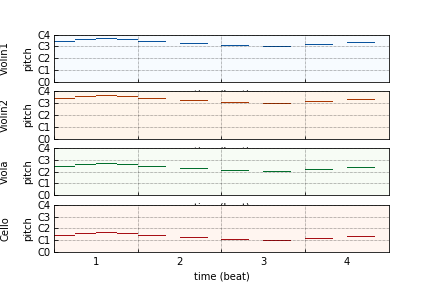
\includegraphics[width=\linewidth]{first_bar.png}
  \caption{Pianoroll visualization of the first measure of
    Beethoven's Serioso String Quartet in F Minor}
  \label{pianoroll}
  \Description{A pianoroll representation of cello, viola and violin
    parts from a Beethoven piece.}
\end{figure}

\begin{figure}[h]
  \centering
  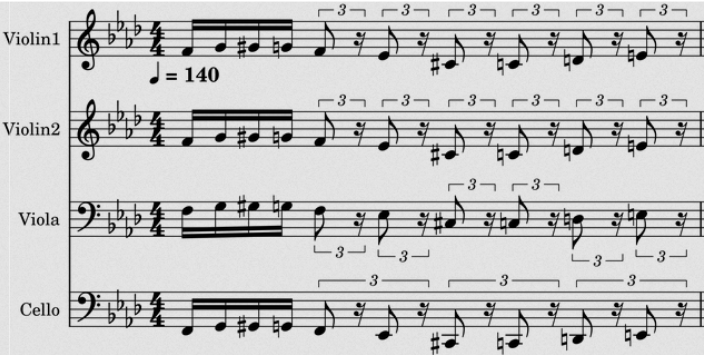
\includegraphics[width=\linewidth]{first_bar_sheet.png}
  \caption{Sheet music of the first measure of Beethoven's Serioso
    String Quartet in F Minor}
  \label{sheet}
  \Description{A measure of sheet music cello, viola, and violin parts
    from Beethoven piece.}
\end{figure}


Data augmentation is also possible and we assess its impact on
the results--the literature suggests augmentation via pitch shifting
each training example up or down by up to six semitones, and
increasing or reducing the speed by up to 10\% in order to create
additional training examples and reduce overfitting
\cite{oore_this_2018}.

The multi-stream representation discussed in
\cite{kumar2019polyphonic} addresses the issue of extreme class
imbalance and sparsity in the pianoroll representation.

\subsection{Model Design}

The model is a recurrent variational autoencoder; both Long Short-Term
Memory (LSTM) and Gated Recurrent Unit (GRU) cell types were tested.

The encoder model utilizes an embedding layer to encode the note pitch
integers as vectors; embedding vector length is a tunable
hyperparameter and we found the best results with it set to 8. Then
two LSTM layers, with a dropout layer in between, convert the
sequences into latent codes, which are modeled as a multidimensional
Gaussian distribution.

The decoder model samples from the latent space $z$ with the
distribution parameterized by the $\mu$ and $log(\sigma)$ values
learned by the encoder.

TODO: model architecture plots

\subsection{Model Evaluation}

Evaluation of generative models is challenging because there is no
equivalent of an accuracy metric like what is used in supervised
learning. For autoencoder models we can measure how accurately the
model can reconstruct its own inputs, but this does not tell us the
quality of the interpolated examples. Generative models are typically
evaluated using a combination of qualitative metrics whereby human
judges rate the quality of the generated examples (essentially a
Turing test), and quantitative metrics that assess the differences in
the parametric distributions of generated and real examples. Yang and
Lerch (2020) proposes a set of metrics informed by music theory, for
probabilistically evaluating how similar the generations are to known
sample distributions of real music \cite{yang_evaluation_2020}. These
metrics include counts, ranges, histograms and transition matrices of
pitches and note lengths, then the Kullback-Leibler divergence and
overlapping area of the probability density functions are used to
compare against known reference distributions per musical genre
\cite{yang_evaluation_2020}. Due to the cost and time requirements
associated with designing a human subjects experiment, we
utilize this quantitative approach to the quality assessment of
generated samples.

\section{Results}

TODO: learning curve plot



\section{Discussion}

\bibliographystyle{ACM-Reference-Format}
\bibliography{paper}

\end{document}
\endinput
